\chapter{Introduction}
\label{cha:introduction}
As cities grow, efficient public transport systems
are becoming increasingly important. To offer a more efficient
service, public transport providers use systems
that predict arrival times of buses, trains and similar vehicles,
and present this information to the general public. The accuracy
and reliability of these predictions are paramount, since many
people depend on them, and erroneous predictions reflect badly on the
public transport provider.

Machine learning algorithms have been applied with great
promise to predict arrival times~\cite{kim2017probabilistic, 
  pang2018learning, Nguyen2018Jun}, and research is still ongoing.
Modern approaches have seen heavy use of Recurrent Neural Networks
(RNNs) to directly model arrival times from the current state of public
transport vehicles, an approach which has shown very good prediction accuracy
but has major drawbacks:

\begin{enumerate}
\item It does not quantify prediction uncertainties.
\item It is severely lacking in explainability.
\end{enumerate}

To make good decisions based of model predictions, it is important to 
know the prediction uncertainty. Being able to explain how
a model makes its predictions is also a extremely desirable,
since it allows reasoning about why a model made a certain prediction,
and about how a model would act in previously unseen
scenarios. 
To address the first problem, a generative model can be used instead
of RNNs. However, solving the second problem and achieving a satisfying
level of explainability requires a much richer model of the data altogether.
One promising approach to create such a model is \textit{motion
  pattern learning} (or \textit{trajectory learning}), where the goal is to learn a \textit{motion
  pattern} (also known as \textit{activity
  pattern} or \textit{activity model})
which represents a cluster of individually observed
trajectories. Motion pattern learning is a problem which spans several
fields, such as computer vision~\cite{Morris2008Sep, Zhang2006Aug,
  Kim2011Nov, Campo2017Aug}, pattern recognition~\cite{Tang2018Aug}, autonomous 
vehicles~\cite{Goli2018Jun}, and health
informatics~\cite{Pimentel2013Sep}, and is like arrival time
prediction an active area of research.

By combining motion pattern learning and generative modeling,
it is possible to make sophisticated predictions, and gain a lot of
insight on how the system performs. For instance, it would be
possible to present the probability of arriving on time, in
real-time, to passengers planning trips with several transits.
The public transport provider could see routes where
predictions are particularly inaccurate, and analyse the motion
patterns on those routes, to help explain their poor performance. 
The motion patterns could be automatically analysed for
detecting events of interest, such as ``velocity change from 50 to 40
km/h'', ``stop'', ``queue'', ``emergency break'', to help explain the
bad predictions. They could also be processed for anomaly
detection, to automatically detect if stations are missed or if public
transport vehicles stray from the designated route, or stand still for
a long time.
Based on the information extracted, the public transport provider
could make efforts to improve the routes by, for instance, moving routes, moving stops or changing
time schedules. Motion patterns created after the changes have been
made could then be compared to previous ones, to see what effects
the changes had. By iterating this process, continuous improvements
could be made.

%All these things would be impossible using solely point-wise predictions.

%This thesis project aims to tackle both problems by modeling motion
%patterns as Gaussian processes (GPs) and by predicting the arrival
%times using Gaussian Process Regression (GPR). and demonstrate the
%advantages from a business point of view 

%Some of these are Hidden Markov Models
%  (HMMs)~\cite{Morris2008Sep,Suzuki2007Oct}, traditional clustering
%  using Dynamic Time Warping and Longest Common Subsequence~\cite{Tang2018Aug, Vlachos2002Feb},
%  Gaussian Processes~\cite{Tran2014Jun,
%    Pimentel2013Sep, Leysen2016Sep, Campo2017Aug, Tiger2015Jul},
%   and topic modeling~\cite{Wang2011}.
% The advantages of basing predictions of a motion pattern model is numerous, including
% detecting common characteristics, anlaysis of patterns that produce
% erroneous predictions and outlier detection.

\section{Problem Description}
This section addresses the problems that need to be solved to create a
system that both learns motion patterns and makes arrival
time predictions that quantifies uncertainty. It also proposes
solutions to these problems. An illustration of the data flow of the
system can be seen in Figure~\ref{fig:system-subproblems}.
\begin{figure}[H]
  \centering
  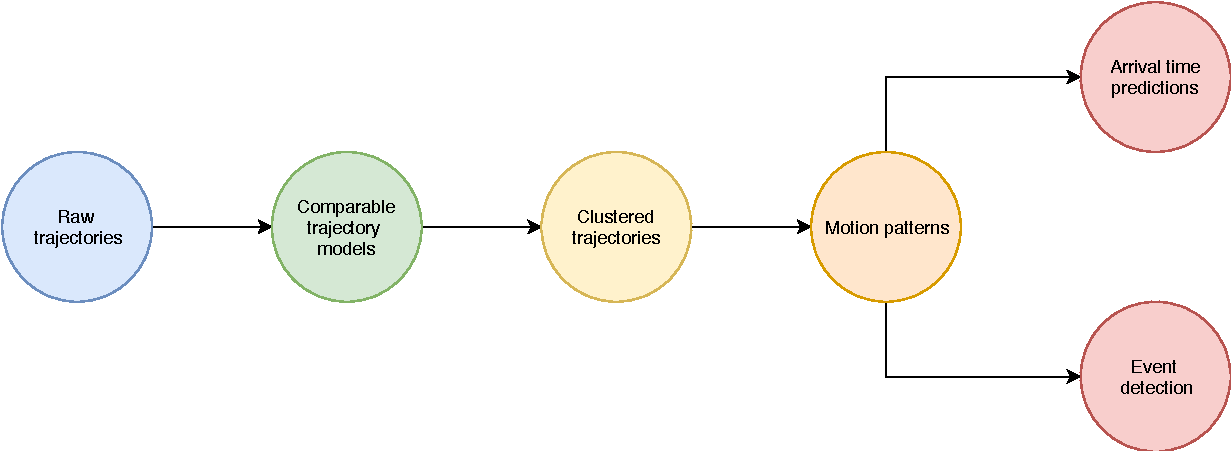
\includegraphics[width=0.7\textwidth]{figures/system-subproblems}
  \caption{An illustration of the data flow in a system that can make
    arrival time predictions and detect events in motion patterns.}\label{fig:system-subproblems}
\end{figure}

\subsection{Trajectory Comparison}
The first step in the system requires a way of comparing
trajectories, which is not straight-forward. The reason for this is that trajectories
can have different lengths and unevenly spaced observations.
The proposed way of doing this is by \textit{synchronising} them,
by modeling the trajectories spatial position as two independent
Gaussian processes (GPs) \(f_x(\tau) \mapsto
x\), \(f_y(\tau) \mapsto y\) for $\tau = [0,1]$, and learning an
inverse GP \(f(x, y) \mapsto \tau\). A similarity
metric for model \(M_k\) is then given by the likelihood \(P(u, v | M_k)\), where
$u$ and $v$ are given by the function compositions \(u = (f_{y} \circ g)(x, y)\),
\(v = (f_{x} \circ g)(x, y)\).

%and then using the likelihood of GP models as a
%similarity metric. The synchronisation step can also be done by GPs,
%so in total the functions $(x, y) \mapsto \tau \mapsto
%x, y$ would be modeled for $\tau = [0,1]$.

\subsection{TrajectoryClustering}
Given a similarity metric, trajectories can be
clustered. Agglomerative clustering is proposed for this task.
One difficult question with clustering is what value of similarity to consider
as ``close''. A lot of manual experiments would be needed to
answer this, which could be very time consuming. Fortunately, the thesis
project can proceed without properly solving this task, as clusters
with a single trajectory can be considered.

\subsection{Motion Pattern Learning}
The challenge after clustering is to find a motion
pattern model $M_k$ that represents trajectories of cluster $k$ well. 
This can be done by fitting a GP
that maximises the likelihood of the cluster data, but also in several
other more sophisticated ways, should time permit. For the case of a single trajectory in
a cluster, this problem is reduced to ordinary Gaussian
process regression (GPR).

\subsection{Arrival Time Prediction}
Once motion patterns have been learned, arrival time $t$ can be predicted
by modeling $P(t | x, y, M_k)$ for observed position $(x, y)$. The proposed solution to this is one GPR
model per motion pattern, combined in a mixture to form the final
predictive distribution
\[P(t | x, y) = \sum_{k} P(t | x, y, M_k)P(M_k | x, y).\]

\subsection{Event Detection}
The final problem is automatically extracting events from motion
patterns. This can be done by asserting a GP for the motion pattern,
and searching over different kernel structures to maximise marginal
likelihood. By searching over kernels which carry a specific meaning (in this case
kernels would correspond to specific events), it is possible to
detect events based on the kernel composition~\cite{duvenaud2013structure}.

\section{Aim}
\label{sec:aim}
The aim of this thesis project is to model motion patterns of public
transport vehicles using Gaussian Processes, and use these
models to make arrival time predictions with an accuracy that is
competitive to current state-of-the-art models~\cite{Sinn2012Sep,
  Gurmu2014, pang2018learning}. Furthermore, the project aims to
detect specific characteristics from motion patterns, such as ``the
driver had to emergency break'', or ``the vehicles speed was very slow'', to see if certain characteristics
are more common in motion patterns where the vehicle is too early or
too late, compared to publicly available time schedules. Finally, this
project aims to investigate how outlier motion patterns can be
detected.

\section{Research questions}
\label{sec:research-questions}

\begin{enumerate}
\item How can Gaussian processes be used to capture trajectory motion
  patterns, such that arrival time predictions based on these patterns minimise MAE?

\item How can similar trajectories be clustered into motion patterns, 
  such that arrival time predictions based on these patterns minimise MAE? 
  
\item How can specific events be automatically detected in a
  motion pattern using compositional kernel search?

\item How can outlier motion patterns be detected?
\end{enumerate}

%Observe that a very specific research question almost always
%leads to a better thesis report than a general research question
%(it is simply much more difficult to make something good
%from a general research question.)

%The best way to achieve a really good and specific research
%question is to conduct a thorough literature review and get
%familiarized with related research and practice. This leads to
%ideas and terminology which allows one to express oneself
%with precision and also have something valuable to say in the
%discussion chapter. And once a detailed research question
%has been specified, it is much easier to establish a suitable
%method and thus carry out the actual thesis work much faster
%than when starting with a fairly general research question. In
%the end, it usually pays off to spend some extra time in the
%beginning working on the literature review. The thesis
%supervisor can be of assistance in deciding when the research
%question is sufficiently specific and well-grounded in related
%research.

\section{Delimitations}
\label{sec:delimitations}
The domain of the thesis project is specifically buses in
Linköping. Data on trains is available, but making the system
work for trains is out of the scope. The thesis project is limited further
to arrival time predictions on consecutive
but stops. Predictions for bus stops several steps ahead will
consequently not be considered.

%The data used is provided by Östgötatrafiken AB and is not publicly
%available. 

%This is where the main delimitations are described. For
%example, this could be that one has focused the study on a
%specific application domain or target user group. In the
%normal case, the delimitations need not be justified.

\section{Report Outline}
